\title[Gate drivers]{Gate drivers for fast switching}
\section{Gate drivers}

\begin{frame}[plain]
	\titlepage
\end{frame}

%%%%%%%%%%%%%%%%%%%%%%%%%%%%%%%%%%%%%%%%%%%%%%%%%%%%%%%%%%%%%
%% Overview %%
%%%%%%%%%%%%%%%%%%%%%%%%%%%%%%%%%%%%%%%%%%%%%%%%%%%%%%%%%%%%%
\subsection{Requirements}

\begin{frame}
	\frametitle{Overview}
	L3 made the gate loop short. This lecture is about the circuit that drives it: it must switch a GaN or SiC transistor within a few nanoseconds, every 100\,ns, and keep it off while the other switch turns on.
	\begin{itemize}
		\item Requirements: voltage levels, timing, isolation
		\item Gate-loop dynamics: damping, turn-on and turn-off paths, common-source inductance
		\item False turn-on caused by $\mathrm{d}v/\mathrm{d}t$ and $\mathrm{d}i/\mathrm{d}t$
		\item Driving e-mode GaN, cascode GaN and SiC
		\item Bootstrap supply, isolation and dead time
		\item Gate drive above 10\,MHz
	\end{itemize}
	After this lecture you can select a gate driver for a given transistor and switching frequency, size the gate resistors and the bootstrap capacitor and check the timing budget. The design project starts at the end of the lecture.
\end{frame}

%%%%%%%%%%%%%%%%%%%%%%%%%%%%%%%%%%%%%%%%%%%%%%%%%%%%%%%%%%%%%
%% Functions of a gate driver %%
%%%%%%%%%%%%%%%%%%%%%%%%%%%%%%%%%%%%%%%%%%%%%%%%%%%%%%%%%%%%%
\begin{frame}
	\frametitle{Functions of a gate driver}
	\begin{columns}[T]
		\begin{column}{0.5\textwidth}
			\begin{figure}
				\centering
				\begin{circuitikz}[scale=0.78, transform shape]
					\tikzset{blk/.style={draw, fill=white, minimum height=0.9cm, minimum width=1.3cm, align=center, font=\footnotesize}}
					\draw[densely dashed, gray] (2.1,-1.9) -- (2.1,1.3);
					\node[blk] (pwm) at (0,0) {PWM};
					\node[blk] (iso) at (2.1,0) {level\\shift};
					\node[blk, minimum height=1.3cm] (drv) at (4.2,0) {driver};
					\node[blk] (sup) at (4.2,1.9) {floating\\supply};
					\draw[-{Latex[length=1.6mm]}] (pwm) -- (iso);
					\draw[-{Latex[length=1.6mm]}] (iso) -- (drv);
					\draw[-{Latex[length=1.6mm]}] (sup) -- (drv);
					\draw (drv.east) to[R, l=$R_\mathrm{G}$] ++(1.7,0) coordinate (g);
					\draw (g) node[nigfete, anchor=G] (Q) {};
					\draw (Q.D) -- ++(0,0.5) node[above] {$V_\mathrm{DC}$};
					\draw (Q.S) -- (Q.S |- 0,-1.6) coordinate (sw) node[circ]{} -- ++(0.7,0) node[right] {$v_\mathrm{sw}$};
					\draw (drv.south) -- (drv.south |- sw) -- (sw);
					\node[font=\scriptsize, anchor=north east] at (2.0,-1.3) {ground};
					\node[font=\scriptsize, anchor=north west] at (2.2,-1.3) {switch node};
				\end{circuitikz}
				\caption{High-side gate drive (simplified)}
			\end{figure}
		\end{column}
		\begin{column}{0.47\textwidth}
			\footnotesize
			\begin{itemize}
				\item Shift the logic signal from ground to the source of the switch. For the high-side switch this is the switch node, which moves by $V_\mathrm{DC}$ within nanoseconds.
				\item Deliver amperes for nanoseconds: $5\,\mathrm{V}/2\,\Omega=2.5$\,A peak, but on average only $Q_\mathrm{G}f_\mathrm{sw}=59$\,mA (EPC2045, 10\,MHz). A capacitor at the driver pins supplies the peaks.
				\item Hold the switch off while the other switch turns on.
				\item Protect: undervoltage lockout (UVLO), over-current, over-temperature.
				\item Provide a floating supply for the high-side driver, referred to the switch node.
			\end{itemize}
		\end{column}
	\end{columns}
	\blfootnote{Sources: Perreault, MIT 6.622, Lecture 38, 2023; Lidow et al., 2019, Ch.\ 3.}
\end{frame}

%%%%%%%%%%%%%%%%%%%%%%%%%%%%%%%%%%%%%%%%%%%%%%%%%%%%%%%%%%%%%
%% Gate drive voltages %%
%%%%%%%%%%%%%%%%%%%%%%%%%%%%%%%%%%%%%%%%%%%%%%%%%%%%%%%%%%%%%
\begin{frame}
	\frametitle{Gate drive voltages}
	\begin{table}
		\centering
		\footnotesize
		\begin{tabular}{|l|l|l|l|}
			\hline
			\textbf{Device}           & \textbf{Example} & \textbf{Recommended on / off}                  & \textbf{Absolute maximum} \\
			\hline
			Si MOSFET                 & --               & 10--12\,V / 0\,V                               & $\pm20$\,V                \\
			SiC MOSFET, generation 2  & C2M0280120D      & $+20$\,V / $-5$\,V                             & $+25$\,V / $-10$\,V       \\
			SiC MOSFET, generation 3  & C3M0065090D      & $+15$\,V / $-4$\,V                             & $+19$\,V / $-8$\,V        \\
			e-mode GaN, 100\,V        & EPC2045          & 4--5.25\,V / 0\,V                              & $+6$\,V / $-4$\,V         \\
			e-mode GaN, 650\,V        & GS66516B         & about 6\,V / 0\,V                              & $+7$\,V / $-10$\,V        \\
			GaN GIT, 600\,V           & PGA26E07BA       & gate current, $v_\mathrm{GS}\approx3$--4\,V    & $+4.5$\,V / $-10$\,V      \\
			cascode GaN, 600\,V       & TPH3006PD        & as a Si MOSFET                                 & $\pm18$\,V                \\
			\hline
		\end{tabular}
		\caption{Gate voltages from the datasheets of the examples; GaN after Lidow et al., 2019, Sec.\ 3.2}
	\end{table}
	\small
	\begin{itemize}
		\item e-mode GaN: about 1\,V between the recommended drive and the absolute maximum, so a few hundred mV of gate overshoot matter.
		\item SiC: $R_\mathrm{DS(on)}$ still falls up to the recommended on-voltage. The negative off-voltage gives margin, because $V_\mathrm{th}$ is low and falls with temperature (C3M0065090D: 2.1\,V at 25\,$^\circ$C, 1.6\,V at 150\,$^\circ$C).
		\item Threshold of e-mode GaN: EPC2045 0.8--2.5\,V, typically 1.4\,V.
	\end{itemize}
\end{frame}

%%%%%%%%%%%%%%%%%%%%%%%%%%%%%%%%%%%%%%%%%%%%%%%%%%%%%%%%%%%%%
%% Timing budget %%
%%%%%%%%%%%%%%%%%%%%%%%%%%%%%%%%%%%%%%%%%%%%%%%%%%%%%%%%%%%%%
\begin{frame}
	\frametitle{Timing budget at 10\,MHz}
	\begin{columns}[T]
		\begin{column}{0.52\textwidth}
			\begin{figure}
				\centering
				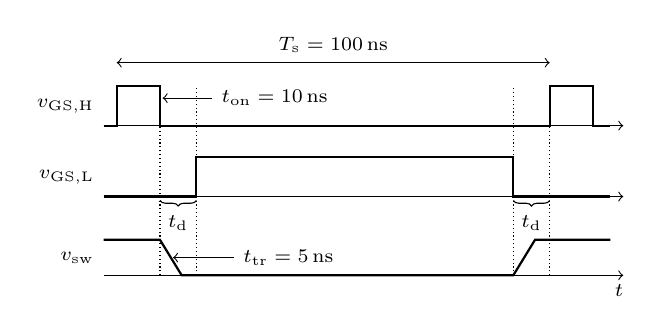
\begin{tikzpicture}[x=0.055cm, y=0.5cm, font=\scriptsize]
					% time axes
					\foreach \y in {0,2.0,3.8} {\draw[->] (-3,\y) -- (117,\y);}
					\node[anchor=east] at (-3,4.3) {$v_\mathrm{GS,H}$};
					\node[anchor=east] at (-3,2.5) {$v_\mathrm{GS,L}$};
					\node[anchor=east] at (-3,0.45) {$v_\mathrm{sw}$};
					\node[anchor=north] at (116,0) {$t$};
					% high-side gate: on 0..10 ns and from 100 ns
					\draw[thick] (-3,3.8) -- (0,3.8) -- (0,4.8) -- (10,4.8) -- (10,3.8) -- (100,3.8) -- (100,4.8) -- (110,4.8) -- (110,3.8) -- (114,3.8);
					% low-side gate: on 18.4..91.6 ns
					\draw[thick] (-3,2.0) -- (18.4,2.0) -- (18.4,3.0) -- (91.6,3.0) -- (91.6,2.0) -- (114,2.0);
					% switch node with 5 ns ZVS transitions
					\draw[thick] (-3,0.9) -- (10,0.9) -- (15,0) -- (91.6,0) -- (96.6,0.9) -- (110,0.9) -- (114,0.9);
					% markers
					\foreach \t in {10,18.4,91.6,100} {\draw[densely dotted] (\t,0) -- (\t,4.8);}
					\draw[<->] (0,5.4) -- node[above] {$T_\mathrm{s}=100$\,ns} (100,5.4);
					\draw[->] (22,4.5) node[right] {$t_\mathrm{on}=10$\,ns} -- (10.6,4.5);
					\draw[decorate, decoration={brace, mirror, amplitude=2pt}] (10,1.9) -- (18.4,1.9) node[pos=0.5, below=2pt] {$t_\mathrm{d}$};
					\draw[decorate, decoration={brace, mirror, amplitude=2pt}] (91.6,1.9) -- (100,1.9) node[pos=0.5, below=2pt] {$t_\mathrm{d}$};
					\draw[->] (27,0.45) node[right] {$t_\mathrm{tr}=5$\,ns} -- (13.0,0.45);
				\end{tikzpicture}
				\caption{ZVS half-bridge at 10\,MHz, $D=0.1$, $t_\mathrm{d}=8.4$\,ns (to scale)}
			\end{figure}
			\begin{block}{Key message}
				At 10\,MHz, timing is part of the power stage.
			\end{block}
		\end{column}
		\begin{column}{0.45\textwidth}
			\small
			\begin{itemize}
				\item On-time of the high-side switch: 10\,ns. The minimum pulse width of the driver must be shorter.
				\item ZVS transition: $2Q_\mathrm{oss}/I_\mathrm{L}=2\cdot25\,\mathrm{nC}/10\,\mathrm{A}=5$\,ns (EPC2045, 48\,V).
				\item Delay mismatch of the two driver channels: $\Delta t_\mathrm{pd}=3.4$\,ns (LMG1210).
				\item $t_\mathrm{d}\geq t_\mathrm{tr}+\Delta t_\mathrm{pd}=8.4$\,ns. The two dead times take 17\,\% of the period.
				\item A propagation delay of 10--35\,ns delays every control action by 0.1--0.35 periods.
			\end{itemize}
		\end{column}
	\end{columns}
\end{frame}

%%%%%%%%%%%%%%%%%%%%%%%%%%%%%%%%%%%%%%%%%%%%%%%%%%%%%%%%%%%%%
%% Poll: driver selection %%
%%%%%%%%%%%%%%%%%%%%%%%%%%%%%%%%%%%%%%%%%%%%%%%%%%%%%%%%%%%%%
% Two pages: question (page 1) and answer (page 2).
\begin{frame}<handout:1-2>
	\frametitle{Driver selection}
	Which driver can operate a 48\,V GaN half-bridge at 10\,MHz with $D=0.1$ and switch-node edges of up to 50\,V/ns? Vote.
	\begin{table}
		\centering
		\small
		\begin{tabular}{|l|l|r|r|r|r|}
			\hline
			  & \textbf{Driver}                          & \textbf{$t_\mathrm{pd}$} & \textbf{Matching} & \textbf{Min.\ pulse} & \textbf{CMTI} \\
			\hline
			A & LMG1205, half-bridge                     & 35\,ns                   & 1.5\,ns           & 10\,ns               & 50\,V/ns      \\
			B & LMG1210, half-bridge                     & 10\,ns                   & 3.4\,ns           & 4\,ns                & 300\,V/ns     \\
			C & ADuM4120, isolated, one channel          & 57--66\,ns               & --                & 50\,ns               & 150\,V/ns     \\
			\hline
		\end{tabular}
		\caption{Typical delays and matching; CMTI of the ADuM4120 is its minimum}
	\end{table}
	\onslide<2-|handout:2>{
		\begin{block}{Answer: B}
			C fails: its minimum pulse width of 50\,ns is five times the on-time of 10\,ns. A has no margin: 10\,ns minimum pulse and 50\,V/ns CMTI, while ringing makes the peak $\mathrm{d}v/\mathrm{d}t$ higher than the average. B meets both with margin; its delay matching of 3.4\,ns enters the dead time.
		\end{block}
	}
	\blfootnote{Sources: TI product pages LMG1205 and LMG1210; ADI ADuM4120 datasheet; Lidow et al., 2019, Tab.\ 3.3 (minimum pulse width and CMTI of the LMG1205).}
\end{frame}

%%%%%%%%%%%%%%%%%%%%%%%%%%%%%%%%%%%%%%%%%%%%%%%%%%%%%%%%%%%%%
%% Gate-loop dynamics %%
%%%%%%%%%%%%%%%%%%%%%%%%%%%%%%%%%%%%%%%%%%%%%%%%%%%%%%%%%%%%%
\subsection{Gate-loop dynamics}

\begin{frame}
	\frametitle{Gate loop as an RLC circuit}
	\begin{columns}[T]
		\begin{column}{0.47\textwidth}
			\begin{figure}
				\centering
				\begin{circuitikz}[scale=0.68, transform shape]
					\draw (0,0) to[sqV, l=$v_\mathrm{dr}$] (0,2.2) to[R, l=$R_\mathrm{dr}$] (2.2,2.2) to[R, l=$R_\mathrm{G,ext}$] (4.4,2.2) to[L, l=$L_\mathrm{G}$] (6.6,2.2) to[R, l=$R_\mathrm{G,int}$] (6.6,0.6) to[C, l=$C_\mathrm{iss}$] (6.6,-0.9) -- (0,-0.9) -- (0,0);
				\end{circuitikz}
				\caption{Gate loop; $L_\mathrm{G}$ includes driver, traces and package}
			\end{figure}
			\small
			$\omega_0=1/\sqrt{L_\mathrm{G}C_\mathrm{iss}}$,\quad $\zeta=\frac{R_\mathrm{G}}{2}\sqrt{C_\mathrm{iss}/L_\mathrm{G}}$,\quad $R_\mathrm{G}=R_\mathrm{dr}+R_\mathrm{G,ext}+R_\mathrm{G,int}$.\\[0.4em]
			No overshoot ($\zeta\geq1$) for
			\begin{equation*}
				R_\mathrm{G}\geq2\sqrt{L_\mathrm{G}/C_\mathrm{iss}}
			\end{equation*}
		\end{column}
		\begin{column}{0.5\textwidth}
			\begin{figure}
				\centering
				\begin{tikzpicture}
					\begin{axis}[
							width=\linewidth, height=5.0cm,
							xmin=0, xmax=15, ymin=0, ymax=8,
							xlabel={Time (ns)}, ylabel={$v_\mathrm{GS}$ (V)},
							grid=major, grid style={gray!20},
							tick label style={font=\scriptsize}, label style={font=\footnotesize},
							legend style={font=\tiny, at={(0.5,1.08)}, anchor=south, legend columns=2, /tikz/every even column/.append style={column sep=0.3cm}}, legend cell align=left,
						]
						\addplot[black, thick] table[x=t, y=r10] {fig/lec04/gate_step.dat};
						\addlegendentry{$R_\mathrm{G}=1\,\Omega$, $\zeta=0.22$}
						\addplot[black, thick, densely dashed] table[x=t, y=r22] {fig/lec04/gate_step.dat};
						\addlegendentry{$R_\mathrm{G}=2.2\,\Omega$, $\zeta=0.49$}
						\addplot[gray, thick] table[x=t, y=r45] {fig/lec04/gate_step.dat};
						\addlegendentry{$R_\mathrm{G}=4.5\,\Omega$, $\zeta=1$}
						\addplot[black, densely dotted, domain=0:15, samples=2] {6};
						\addlegendentry{absolute maximum, 6\,V}
					\end{axis}
				\end{tikzpicture}
				\caption{Ideal 5\,V step, $L_\mathrm{G}=3$\,nH, $C_\mathrm{iss}=600$\,pF}
			\end{figure}
		\end{column}
	\end{columns}
	\blfootnote{Source: Lidow et al., 2019, Sec.\ 3.3, Eq.\ (3.1), written there with $C_\mathrm{GS}$.}
\end{frame}

%%%%%%%%%%%%%%%%%%%%%%%%%%%%%%%%%%%%%%%%%%%%%%%%%%%%%%%%%%%%%
%% Your turn: critical gate resistance %%
%%%%%%%%%%%%%%%%%%%%%%%%%%%%%%%%%%%%%%%%%%%%%%%%%%%%%%%%%%%%%
% Two pages: task (page 1) and task with solution (page 2).
\begin{frame}<handout:1-2>
	\frametitle{Critical gate resistance}
	\begin{block}{Task (5 minutes)}
		A GaN transistor with $C_\mathrm{iss}=600$\,pF and an absolute maximum gate voltage of 6\,V is driven from a 5\,V driver. The gate loop has $L_\mathrm{G}=3$\,nH.
		\begin{enumerate}
			\item Which total gate resistance gives critical damping? Which rise time results?
			\item Is $R_\mathrm{G}=2.2\,\Omega$ acceptable?
			\item How can the gate be switched faster without overshoot?
		\end{enumerate}
	\end{block}
	\onslide<2-|handout:2>{
		\begin{enumerate}
			\item $R_\mathrm{G}=2\sqrt{L_\mathrm{G}/C_\mathrm{iss}}=4.5\,\Omega$. The critically damped step response rises from 10 to 90\,\% in $3.36\sqrt{L_\mathrm{G}C_\mathrm{iss}}=4.5$\,ns.
			\item $\zeta=0.49$, overshoot 17\,\%: peak 5.85\,V and rise time 2.2\,ns. With the driver supply at its upper tolerance of 5.25\,V the peak is 6.1\,V. Not acceptable as a worst case.
			\item Only with a smaller $L_\mathrm{G}$: at critical damping the rise time scales with $\sqrt{L_\mathrm{G}}$. With 1\,nH: $R_\mathrm{G}=2.6\,\Omega$, 2.6\,ns.
		\end{enumerate}
		{\small The ideal step is the worst case; the finite rise time of a real driver output reduces the overshoot.}
	}
\end{frame}

%%%%%%%%%%%%%%%%%%%%%%%%%%%%%%%%%%%%%%%%%%%%%%%%%%%%%%%%%%%%%
%% Turn-on and turn-off paths %%
%%%%%%%%%%%%%%%%%%%%%%%%%%%%%%%%%%%%%%%%%%%%%%%%%%%%%%%%%%%%%
\begin{frame}
	\frametitle{Turn-on and turn-off paths}
	\begin{columns}[T]
		\begin{column}{0.44\textwidth}
			\begin{figure}
				\centering
				\begin{circuitikz}[scale=0.8, transform shape]
					% driver output stage with separate pull-up and pull-down pins
					\draw (-0.4,3.6) node[left] {$V_\mathrm{DD}$} -- (0.5,3.6) to[nos] (0.5,2.4) coordinate (oh);
					\draw (oh) -- (1.9,2.4) to[R, l=$R_\mathrm{G,on}$] (3.9,2.4) -- (4.3,2.4) coordinate (a);
					\draw (0.5,1.2) coordinate (ol) to[nos] (0.5,0) coordinate (k);
					\draw (ol) -- (1.9,1.2) to[R, l_=$R_\mathrm{G,off}$] (3.9,1.2) -- (4.3,1.2) coordinate (b);
					\draw (a) -- (b);
					\draw (4.3,1.8) node[circ]{} -- (4.7,1.8) node[nigfete, anchor=G] (Q) {};
					\draw (Q.D) -- ++(0,0.4);
					\draw (Q.S) -- (Q.S |- k) -- (k);
					\draw[densely dashed, gray] (-0.1,-0.25) rectangle (1.0,3.15);
					\node[font=\scriptsize, anchor=north] at (0.45,-0.3) {driver};
					\node[font=\scriptsize, anchor=south west] at (1.0,2.4) {OUTH};
					\node[font=\scriptsize, anchor=south west] at (1.0,1.2) {OUTL};
				\end{circuitikz}
				\caption{Driver with split outputs}
			\end{figure}
		\end{column}
		\begin{column}{0.53\textwidth}
			\footnotesize
			\begin{itemize}
				\item \textbf{Turn-on}: $R_\mathrm{G,on}$ sets $\mathrm{d}v/\mathrm{d}t$ and $\mathrm{d}i/\mathrm{d}t$, i.e.\ loss against overshoot and EMI. Plateau time (L2) $t_\mathrm{vf}\approx R_\mathrm{G}Q_\mathrm{GD}/(V_\mathrm{dr}-V_\mathrm{pl})$. EPC2045 at 50\,V, $V_\mathrm{pl}\approx2.5$\,V: $R_\mathrm{G}=2.7\,\Omega$ (driver and internal) gives 0.9\,ns ($\approx$\,60\,V/ns), 4.7\,$\Omega$ gives 1.5\,ns ($\approx$\,33\,V/ns).
				\item \textbf{Turn-off}: small $R_\mathrm{G,off}$. If the channel closes before $v_\mathrm{DS}$ rises, the load current charges the output capacitances; the turn-off is almost lossless (L2).
				\item The turn-off loop does not contain the driver supply capacitor and tolerates negative undershoot. It must not ring back above $V_\mathrm{th}$.
				\item Split outputs (separate pins for turn-on and turn-off), e.g.\ LMG1205: 2.1\,$\Omega$ pull-up, 0.6\,$\Omega$ pull-down. With a single output, a diode in parallel with $R_\mathrm{G,on}$ creates the separate off path.
			\end{itemize}
		\end{column}
	\end{columns}
	\blfootnote{Sources: Lidow et al., 2019, Sec.\ 3.3 and 3.5.1; EPC2045 datasheet; TI LMG1205 product page.}
\end{frame}

%%%%%%%%%%%%%%%%%%%%%%%%%%%%%%%%%%%%%%%%%%%%%%%%%%%%%%%%%%%%%
%% Common-source inductance %%
%%%%%%%%%%%%%%%%%%%%%%%%%%%%%%%%%%%%%%%%%%%%%%%%%%%%%%%%%%%%%
\begin{frame}
	\frametitle{Speed limit from $L_\mathrm{CS}$}
	\begin{columns}[T]
		\begin{column}{0.52\textwidth}
			\small
			L2: $v_\mathrm{GS}=v_\mathrm{dr}-R_\mathrm{G}i_\mathrm{G}-L_\mathrm{CS}\,\mathrm{d}i_\mathrm{D}/\mathrm{d}t$. During the current rise, $i_\mathrm{D}\approx g_\mathrm{m}(v_\mathrm{GS}-V_\mathrm{th})$ and $i_\mathrm{G}\approx C_\mathrm{iss}\,\mathrm{d}v_\mathrm{GS}/\mathrm{d}t$:
			\begin{equation*}
				V_\mathrm{dr}-v_\mathrm{GS}=\left(R_\mathrm{G}C_\mathrm{iss}+L_\mathrm{CS}\,g_\mathrm{m}\right)\frac{\mathrm{d}v_\mathrm{GS}}{\mathrm{d}t}
			\end{equation*}
			$L_\mathrm{CS}$ acts like an additional gate resistance $L_\mathrm{CS}\,g_\mathrm{m}/C_\mathrm{iss}$.\\[0.4em]
			Example: $g_\mathrm{m}\approx9$\,S (10\,A at $V_\mathrm{pl}=2.5$\,V, $V_\mathrm{th}=1.4$\,V), $C_\mathrm{iss}=0.74$\,nF. Then 1\,nH acts like 12\,$\Omega$, several times the resistance of the whole gate loop.
		\end{column}
		\begin{column}{0.45\textwidth}
			\small
			Even for $R_\mathrm{G}\rightarrow0$ the current slope is limited: $\mathrm{d}i_\mathrm{D}/\mathrm{d}t=(V_\mathrm{dr}-v_\mathrm{GS})/L_\mathrm{CS}$.
			\begin{table}
				\centering
				\footnotesize
				\begin{tabular}{|r|r|r|}
					\hline
					$L_\mathrm{CS}$ & $\mathrm{d}i/\mathrm{d}t$ at $V_\mathrm{pl}$ & time for 10\,A \\
					\hline
					1\,nH           & 2.5\,A/ns                                    & 4\,ns          \\
					0.2\,nH         & 12.5\,A/ns                                   & 0.8\,ns        \\
					0.1\,nH         & 25\,A/ns                                     & 0.4\,ns        \\
					\hline
				\end{tabular}
				\caption{$V_\mathrm{dr}=5$\,V, $v_\mathrm{GS}=V_\mathrm{pl}=2.5$\,V, $R_\mathrm{G}\rightarrow0$}
			\end{table}
			\begin{block}{Key message}
				With a Kelvin source the gate loop returns at the source pad; only the inductance inside the package remains common.
			\end{block}
		\end{column}
	\end{columns}
	\blfootnote{The exact solution with $g_\mathrm{m}=9$\,S gives 3.3\,ns instead of 4\,ns for 1\,nH. Source: Lidow et al., 2019, Sec.\ 3.6.1.}
\end{frame}

%%%%%%%%%%%%%%%%%%%%%%%%%%%%%%%%%%%%%%%%%%%%%%%%%%%%%%%%%%%%%
%% False turn-on %%
%%%%%%%%%%%%%%%%%%%%%%%%%%%%%%%%%%%%%%%%%%%%%%%%%%%%%%%%%%%%%
\subsection{False turn-on}

\begin{frame}
	\frametitle{Miller turn-on}
	\begin{columns}[T]
		\begin{column}{0.44\textwidth}
			\begin{figure}
				\centering
				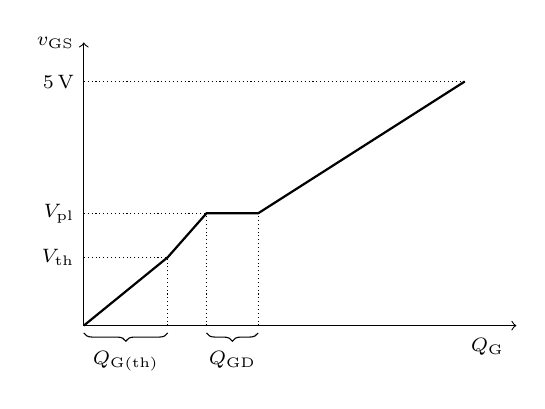
\begin{tikzpicture}[x=0.82cm, y=0.62cm, font=\scriptsize]
					\draw[->] (0,0) -- (6.7,0) node[below left=1pt] {$Q_\mathrm{G}$};
					\draw[->] (0,0) -- (0,5.8) node[left] {$v_\mathrm{GS}$};
					\draw[thick] (0,0) -- (1.3,1.4) -- (1.9,2.3) -- (2.7,2.3) -- (5.9,5.0);
					\draw[densely dotted] (1.3,0) -- (1.3,1.4) -- (0,1.4) node[left] {$V_\mathrm{th}$};
					\draw[densely dotted] (0,2.3) node[left] {$V_\mathrm{pl}$} -- (1.9,2.3);
					\draw[densely dotted] (1.9,0) -- (1.9,2.3);
					\draw[densely dotted] (2.7,0) -- (2.7,2.3);
					\draw[densely dotted] (0,5.0) node[left] {5\,V} -- (5.9,5.0);
					\draw[decorate, decoration={brace, mirror, amplitude=3pt}] (0,-0.15) -- (1.3,-0.15) node[midway, below=3pt] {$Q_\mathrm{G(th)}$};
					\draw[decorate, decoration={brace, mirror, amplitude=3pt}] (1.9,-0.15) -- (2.7,-0.15) node[midway, below=3pt] {$Q_\mathrm{GD}$};
				\end{tikzpicture}
				\caption{Gate charge (schematic). EPC2045 at 50\,V: $Q_\mathrm{G(th)}=1.3$\,nC, $Q_\mathrm{GD}=0.8$\,nC, $Q_\mathrm{G}=5.9$\,nC}
			\end{figure}
		\end{column}
		\begin{column}{0.53\textwidth}
			\footnotesize
			When the other switch turns on, $v_\mathrm{DS}$ of the off-state switch rises and $C_\mathrm{GD}$ pushes charge into its gate.
			\begin{itemize}
				\item Worst case, gate open: the charge $Q_\mathrm{GD}$ must not lift the gate to $V_\mathrm{th}$. A Miller ratio
				      \begin{equation*}
					      Q_\mathrm{GD}/Q_\mathrm{G(th)}<1
				      \end{equation*}
				      guarantees immunity, whatever the driver does.
				\item EPC2045: $0.8/1.3=0.62$ at 50\,V, immune up to its rated 100\,V. The older EPC2016 is sensitive above 40\,\% of its rating, the 650\,V GS66516B at even lower voltage.
				\item Ratio above 1: the off path must carry the current $C_\mathrm{GD}\,\mathrm{d}v/\mathrm{d}t$ without lifting the gate (L3). At the frequency of the edge the gate-loop inductance adds to $R_\mathrm{G,off}$: 2\,nH at 300\,MHz are 3.8\,$\Omega$.
			\end{itemize}
		\end{column}
	\end{columns}
	\blfootnote{Source: Lidow et al., 2019, Sec.\ 2.5, 3.5.2 and Fig.\ 3.10.}
\end{frame}

%%%%%%%%%%%%%%%%%%%%%%%%%%%%%%%%%%%%%%%%%%%%%%%%%%%%%%%%%%%%%
%% di/dt-induced spikes %%
%%%%%%%%%%%%%%%%%%%%%%%%%%%%%%%%%%%%%%%%%%%%%%%%%%%%%%%%%%%%%
\begin{frame}
	\frametitle{Spikes and shoot-through}
	\begin{columns}[T]
		\begin{column}{0.5\textwidth}
			\begin{figure}
				\centering
				\begin{tikzpicture}
					\begin{axis}[
							width=\linewidth, height=4.9cm,
							xmin=0, xmax=16, ymin=-4, ymax=2.5,
							xlabel={Time (ns)}, ylabel={$v_\mathrm{GS}$ (V)},
							grid=major, grid style={gray!20},
							tick label style={font=\scriptsize}, label style={font=\footnotesize},
							legend style={font=\tiny}, legend pos=south east, legend cell align=left,
						]
						\fill[gray!15] (axis cs:2,-4) rectangle (axis cs:3,2.5);
						\addplot[black, thick] table[x=t, y=vu] {fig/lec04/csi_spike.dat};
						\addlegendentry{$R=0.8\,\Omega$, $\zeta=0.22$}
						\addplot[black, thick, densely dashed] table[x=t, y=vd] {fig/lec04/csi_spike.dat};
						\addlegendentry{$R=2.5\,\Omega$, $\zeta=0.68$}
						\addplot[black, densely dotted, domain=0:16, samples=2] {1.4};
						\addlegendentry{$V_\mathrm{th}$}
					\end{axis}
				\end{tikzpicture}
				\caption{Off-state switch: $L_\mathrm{CS}=0.5$\,nH, 10\,A transferred in 1\,ns (shaded), gate loop 2\,nH and 600\,pF}
			\end{figure}
		\end{column}
		\begin{column}{0.47\textwidth}
			\small
			\begin{itemize}
				\item In the dead time the off-state switch conducts the load current in reverse.
				\item The other switch turns on and takes over the current. Its change in $L_\mathrm{CS}$ of the off-state switch drives the gate negative: $-L_\mathrm{CS}\,\mathrm{d}i/\mathrm{d}t=-5$\,V for 1\,ns.
				\item An under-damped gate loop rings back above $V_\mathrm{th}$: shoot-through. The $\mathrm{d}v/\mathrm{d}t$ of the following voltage transition adds Miller charge.
				\item Remedies: Kelvin source, which removes $L_\mathrm{CS}$ from the gate loop, and damping of the off path. A larger $R_\mathrm{G,off}$ damps, but slows the turn-off.
			\end{itemize}
		\end{column}
	\end{columns}
	\blfootnote{Source: Lidow et al., 2019, Sec.\ 3.6.2 and Fig.\ 3.15. Waveforms computed for this lecture.}
\end{frame}

%%%%%%%%%%%%%%%%%%%%%%%%%%%%%%%%%%%%%%%%%%%%%%%%%%%%%%%%%%%%%
%% Remedies %%
%%%%%%%%%%%%%%%%%%%%%%%%%%%%%%%%%%%%%%%%%%%%%%%%%%%%%%%%%%%%%
\begin{frame}
	\frametitle{Keeping the switch off}
	\begin{table}
		\centering
		\footnotesize
		\begin{tabular}{|>{\raggedright\arraybackslash}p{4.4cm}|>{\raggedright\arraybackslash}p{4.4cm}|>{\raggedright\arraybackslash}p{4.6cm}|}
			\hline
			\textbf{Measure}                                                   & \textbf{Effect}                                            & \textbf{Price}                                                                         \\
			\hline
			Device with Miller ratio $<1$                                      & immune to $\mathrm{d}v/\mathrm{d}t$ without help           & choice of device                                                                       \\
			Short, low-resistance off path; Kelvin source                      & shunts $C_\mathrm{GD}\,\mathrm{d}v/\mathrm{d}t$, no $L_\mathrm{CS}$ step & layout effort                                                    \\
			Miller clamp: switch from gate to source inside the driver         & very low impedance after turn-off                          & extra pin; offered by many isolated drivers                                            \\
			Negative off-voltage                                               & margin to $V_\mathrm{th}$                                  & GaN: $V_\mathrm{SD}$ rises by $|v_\mathrm{GS,off}|$; SiC: threshold drift; extra supply \\
			Turn-on of the other switch in the negative dip of the gate voltage & more charge needed for a false turn-on                    & needs fixed timing                                                                     \\
			Slower $\mathrm{d}v/\mathrm{d}t$ (larger $R_\mathrm{G,on}$ of the other switch) & less injected current                         & more switching loss                                                                    \\
			\hline
		\end{tabular}
	\end{table}
	First check the Miller ratio of the device, then design the off path for the frequency content of the edges: hundreds of MHz.
	\blfootnote{Source: Lidow et al., 2019, Sec.\ 3.5 and 3.6.}
\end{frame}

%%%%%%%%%%%%%%%%%%%%%%%%%%%%%%%%%%%%%%%%%%%%%%%%%%%%%%%%%%%%%
%% Device-specific drive %%
%%%%%%%%%%%%%%%%%%%%%%%%%%%%%%%%%%%%%%%%%%%%%%%%%%%%%%%%%%%%%
\subsection{Device-specific drive}

\begin{frame}
	\frametitle{Driving e-mode GaN}
	\textbf{Schottky-type p-GaN gate} (e.g.\ EPC, GaN Systems)
	\begin{itemize}
		\item Voltage drive: 5--6\,V on, 0\,V off; the gate behaves like a capacitor.
		\item Only about 1\,V margin to the absolute maximum: damp the gate loop near critically, regulate the driver supply, control the bootstrap voltage.
		\item Low threshold (EPC2045: 1.4\,V): the off path needs a low impedance, so that coupled currents cannot lift the gate.
		\item Turn off with 0\,V where possible. A negative off-voltage raises $V_\mathrm{SD}$ in the dead time by the same amount, and with it the dead-time loss.
	\end{itemize}
	\begin{block}{Key message}
		The e-mode GaN gate is fast and sensitive: every part of the gate loop is designed, not just the driver.
	\end{block}
	\blfootnote{Source: Lidow et al., 2019, Sec.\ 3.2--3.3.}
\end{frame}

%%%%%%%%%%%%%%%%%%%%%%%%%%%%%%%%%%%%%%%%%%%%%%%%%%%%%%%%%%%%%
%% Driving GIT %%
%%%%%%%%%%%%%%%%%%%%%%%%%%%%%%%%%%%%%%%%%%%%%%%%%%%%%%%%%%%%%
\begin{frame}
	\frametitle{Driving a gate injection transistor}
	\begin{columns}[T]
		\begin{column}{0.45\textwidth}
			\begin{figure}
				\centering
				\begin{circuitikz}[scale=0.8, transform shape]
					\draw (0,0) to[sqV, l=$0/V_\mathrm{P}$] (0,2.0) -- (0.6,2.0) coordinate (a);
					\draw (a) -- (0.6,3.1) to[R, l=$R_\mathrm{G2}$] (4.4,3.1) -- (4.4,2.0) coordinate (g);
					\draw (a) to[R, l_=$R_\mathrm{G1}$] (2.5,2.0) to[C, l_=$C_\mathrm{SU}$] (g);
					\draw (g) node[circ]{} -- (4.8,2.0) node[nigfete, anchor=G] (Q) {};
					\draw (Q.D) -- ++(0,0.3);
					\draw (Q.S) -- (Q.S |- 0,-0.5) -- (0,-0.5) -- (0,0);
				\end{circuitikz}
				\caption{RC drive of a GIT: speed-up branch $R_\mathrm{G1}$--$C_\mathrm{SU}$, holding branch $R_\mathrm{G2}$}
			\end{figure}
		\end{column}
		\begin{column}{0.52\textwidth}
			\small
			In a GIT the gate behaves like a diode, clamped at $V_\mathrm{GS,ss}\approx3$--4\,V; a few mA keep the transistor on. The driver output switches between 0 and $V_\mathrm{P}$.
			\begin{itemize}
				\item Turn-on: $C_\mathrm{SU}$ is still discharged, so a large current flows through $R_\mathrm{G1}$, $I_\mathrm{G,pk}\approx V_\mathrm{P}/R_\mathrm{G1}$, decaying with $\tau=R_\mathrm{G1}C_\mathrm{SU}$.
				\item On-state: $R_\mathrm{G2}$ supplies the holding current $I_\mathrm{G,ss}=(V_\mathrm{P}-V_\mathrm{GS,ss})/R_\mathrm{G2}$.
				\item Turn-off: the charge on $C_\mathrm{SU}$ pulls the gate negative and speeds up the turn-off.
			\end{itemize}
		\end{column}
	\end{columns}
	\blfootnote{Source: Lidow et al., 2019, Sec.\ 3.4, Fig.\ 3.6 and 3.7.}
\end{frame}

%%%%%%%%%%%%%%%%%%%%%%%%%%%%%%%%%%%%%%%%%%%%%%%%%%%%%%%%%%%%%
%% Cascode GaN and SiC %%
%%%%%%%%%%%%%%%%%%%%%%%%%%%%%%%%%%%%%%%%%%%%%%%%%%%%%%%%%%%%%
\begin{frame}
	\frametitle{Cascode GaN and SiC}
	\begin{columns}[T]
		\begin{column}{0.48\textwidth}
			\begin{minipage}[t]{0.36\linewidth}
				\vspace{0pt}
				\centering
				\begin{circuitikz}[scale=0.62, transform shape]
					\draw (0,3.2) node[nigfetd] (J) {};
					\draw (J.D) -- ++(0,0.3) node[above] {D};
					\draw (J.S) -- ++(0,-0.3) coordinate (m);
					\draw (m) node[nigfete, anchor=D, xscale=-1] (M) {};
					\draw (M.S) -- ++(0,-0.3) coordinate (s) -- ++(0,-0.3) node[below] {S};
					\draw (J.G) -- ++(-0.4,0) coordinate (jg) -- (jg |- s) -- (s) node[circ]{};
					\draw (M.G) -- ++(0.4,0) node[right] {G};
				\end{circuitikz}
			\end{minipage}\hfill
			\begin{minipage}[t]{0.62\linewidth}
				\vspace{0pt}
				\small\raggedright
				\textbf{Cascode GaN}: depletion-mode GaN (top) in series with a low-voltage Si MOSFET. The driver sees the MOSFET gate: $\pm18$\,V (TPH3006PD), standard drivers.
			\end{minipage}\\[0.5em]
			\small
			\begin{itemize}
				\item Turn-off is driven by the load current, which charges the MOSFET output capacitance.
				\item Two dies, two loops with common inductance (common source, and the connection between the dies). The Si MOSFET limits the turn-on speed; its body diode adds reverse recovery.
			\end{itemize}
		\end{column}
		\begin{column}{0.49\textwidth}
			\small
			\textbf{SiC MOSFET}
			\begin{itemize}
				\item On +15 to +20\,V; off 0 to $-5$\,V for margin against false turn-on.
				\item Threshold drift under gate bias stress (BTI): positive stress raises $V_\mathrm{th}$, negative stress lowers it. Stay within the recommended range (test method: JEDEC JEP184, 2021).
			\end{itemize}
			\textbf{Short circuit}
			\begin{itemize}
				\item Withstand time: Si $\geq10\,\mu$s, SiC about 1\,$\mu$s, GaN 200--600\,ns at 400\,V (longer at lower voltage).
				\item Desaturation protection: total response about 200\,ns (SiC and GaN).
			\end{itemize}
		\end{column}
	\end{columns}
	\blfootnote{Sources: Lidow et al., 2019, Sec.\ 3.11; Wang, Zhang, Jones, 2018, Sec.\ 1.2 and 7.1.}
\end{frame}

%%%%%%%%%%%%%%%%%%%%%%%%%%%%%%%%%%%%%%%%%%%%%%%%%%%%%%%%%%%%%
%% Floating supply and signals %%
%%%%%%%%%%%%%%%%%%%%%%%%%%%%%%%%%%%%%%%%%%%%%%%%%%%%%%%%%%%%%
\subsection{Floating supply and signals}

\begin{frame}
	\frametitle{Bootstrap supply}
	\begin{columns}[T]
		\begin{column}{0.53\textwidth}
			\begin{figure}
				\centering
				\begin{circuitikz}[scale=0.72, transform shape]
					% half-bridge
					\draw (6.2,5.6) node[above] {$V_\mathrm{DC}$} -- (6.2,5.2) node[nigfete, anchor=D] (QH) {};
					\draw (QH.S) -- ++(0,-0.4) coordinate (sw);
					\draw (sw) node[nigfete, anchor=D] (QL) {};
					\draw (QL.S) -- ++(0,-0.3) node[ground] {};
					\draw (sw) node[circ]{} -- ++(1.0,0) node[right] {$v_\mathrm{sw}$};
					% high-side driver
					\node[draw, minimum width=1.3cm, minimum height=1.5cm, anchor=east, align=center, font=\footnotesize] (drv) at ($(QH.G)+(-1.9,0)$) {HS\\driver};
					\draw (drv.east) to[R, l=$R_\mathrm{G}$] (QH.G);
					\draw (drv.south) -- (drv.south |- sw) -- (sw);
					% bootstrap capacitor and diode
					\draw (drv.north) -- ++(0,0.5) coordinate (hb) -- ++(-1.6,0) coordinate (c1);
					\draw (c1) to[C, l_=$C_\mathrm{boot}$] (c1 |- sw) -- (drv.south |- sw);
					\draw ($(c1)+(-2.4,0)$) node[left] {$V_\mathrm{DD}$} to[D, l=$D_\mathrm{boot}$] (c1);
					\draw (QL.G) -- ++(-0.4,0) node[left, font=\footnotesize] {LS driver};
					% reverse conduction in the dead time
					\draw[-{Latex[length=1.6mm]}] ($(QL.S)+(0.75,0.1)$) -- ($(QL.D)+(0.75,-0.1)$) node[midway, right, font=\footnotesize] {$t_\mathrm{d}$};
				\end{circuitikz}
				\caption{$C_\mathrm{boot}$ charges while the low-side switch conducts. Arrow: reverse current in the dead time}
			\end{figure}
		\end{column}
		\begin{column}{0.44\textwidth}
			\footnotesize
			\begin{itemize}
				\item Size: $C_\mathrm{boot}\geq Q_\mathrm{tot}/\Delta V$, with $Q_\mathrm{tot}$ the gate and driver charge per cycle and $\Delta V$ the allowed droop. 8\,nC and 0.1\,V give 80\,nF: use 100\,nF.
				\item Over-charge: while the low-side switch conducts in reverse, the switch node is at $-V_\mathrm{SD}$, and $C_\mathrm{boot}$ charges towards $V_\mathrm{DD}-V_\mathrm{F}+V_\mathrm{SD}=5-0.5+2.5=7$\,V. The diode cannot discharge it, so the charge accumulates over many periods.
				\item Remedies: short dead time, Schottky diode across the low-side switch, clamp, synchronous GaN bootstrap switch (best regulation and efficiency).
				\item $D_\mathrm{boot}$ adds capacitance and recovery charge to the switch node.
			\end{itemize}
		\end{column}
	\end{columns}
	\blfootnote{Sources: Lidow et al., 2019, Sec.\ 3.7 and Tab.\ 3.2; Reusch and de Rooij, IEEE APEC 2017, pp.\ 2459--2466.}
\end{frame}

%%%%%%%%%%%%%%%%%%%%%%%%%%%%%%%%%%%%%%%%%%%%%%%%%%%%%%%%%%%%%
%% Mini-case: bootstrap at 5 MHz %%
%%%%%%%%%%%%%%%%%%%%%%%%%%%%%%%%%%%%%%%%%%%%%%%%%%%%%%%%%%%%%
% Two pages: task (page 1) and task with solution (page 2).
\begin{frame}<handout:1-2>
	\frametitle{Bootstrap at 5\,MHz}
	\begin{block}{Task (5 minutes)}
		A GaN half-bridge runs at 5\,MHz with up to 90\,\% high-side duty cycle: the bootstrap capacitor is recharged in only 20\,ns per period. The high-side driver draws $Q_\mathrm{tot}=8$\,nC per cycle; $C_\mathrm{boot}=100$\,nF, $V_\mathrm{DD}=5$\,V.
		\begin{enumerate}
			\item By how much does the bootstrap voltage drop per cycle?
			\item Which bootstrap voltage results in steady state with a diode path ($V_\mathrm{F}=0.5$\,V, 2\,$\Omega$), and with a synchronous switch (0.5\,$\Omega$)?
		\end{enumerate}
	\end{block}
	\onslide<2-|handout:2>{
		\begin{enumerate}
			\item $\Delta V=Q_\mathrm{tot}/C_\mathrm{boot}=80$\,mV.
			\item The recharge returns 8\,nC within 20\,ns, on average 0.4\,A. As $R_\mathrm{boot}C_\mathrm{boot}=200\,\mathrm{ns}\gg20$\,ns, the current is almost constant: $v_\mathrm{boot}\approx V_\mathrm{DD}-V_\mathrm{F}-Q_\mathrm{tot}R_\mathrm{boot}/t_\mathrm{rech}$.\\
			      Diode: $5-0.5-0.8=3.7$\,V, below the 4\,V needed for full enhancement; the driver may reach its undervoltage lockout. Synchronous switch: $5-0.2=4.8$\,V.
		\end{enumerate}
	}
	\blfootnote{See also: Mehta, TI application report SNVA723A, 2018.}
\end{frame}

%%%%%%%%%%%%%%%%%%%%%%%%%%%%%%%%%%%%%%%%%%%%%%%%%%%%%%%%%%%%%
%% Isolation and CMTI %%
%%%%%%%%%%%%%%%%%%%%%%%%%%%%%%%%%%%%%%%%%%%%%%%%%%%%%%%%%%%%%
\begin{frame}
	\frametitle{Isolation and CMTI}
	\begin{columns}[T]
		\begin{column}{0.46\textwidth}
			\begin{figure}
				\centering
				\begin{circuitikz}[scale=0.6, transform shape]
					\tikzset{blk/.style={draw, minimum height=0.9cm, minimum width=1.3cm, align=center, font=\small}}
					\node[blk] (ctl) at (0,2.6) {PWM};
					\node[blk] (drv) at (4.6,2.6) {driver};
					\draw[-{Latex[length=1.6mm]}] (ctl) -- node[above, font=\small, pos=0.27] {signal} (drv);
					\draw[densely dashed, gray] (2.3,-2.4) -- (2.3,3.6);
					\node[font=\scriptsize, anchor=south] at (2.3,3.6) {isolation};
					\draw (ctl.south) -- (0,0) coordinate (p0);
					\draw (drv.south) -- (4.6,0) coordinate (s0);
					\draw (s0) -- (3.7,0) to[C, i=$i_\mathrm{CM}$] (0.9,0) -- (p0);
					\node[anchor=south west] at (2.5,0.3) {$C_\mathrm{iso}$};
					\draw (s0) node[circ]{} to[sqV, l=$v_\mathrm{sw}$] (4.6,-2.0) coordinate (s1);
					\draw (p0) -- (0,-2.0) node[ground] {};
					\draw (0,-2.0) -- (s1);
					\node[font=\scriptsize, anchor=west] at (4.75,0.3) {switch node};
				\end{circuitikz}
				\caption{Common-mode current through the isolation capacitance}
			\end{figure}
			\small
			$i_\mathrm{CM}=C_\mathrm{iso}\,\mathrm{d}v/\mathrm{d}t$: 2\,pF at 100\,V/ns gives 0.2\,A, 10\,pF 1\,A.
		\end{column}
		\begin{column}{0.51\textwidth}
			\begin{table}
				\centering
				\footnotesize
				\begin{tabular}{|l|r|}
					\hline
					\textbf{Measured peak $\mathrm{d}v/\mathrm{d}t$} & \textbf{V/ns} \\
					\hline
					SiC MOSFET, discrete (CMF20120D)                 & 30            \\
					SiC power module                                 & 80            \\
					e-mode GaN (GS66508P)                            & 100           \\
					\hline
					\textbf{Minimum CMTI of isolators}               &               \\
					\hline
					optocoupler                                      & 30            \\
					capacitive                                       & 100           \\
					magnetic (transformer)                           & 75            \\
					RF-based                                         & 200           \\
					\hline
				\end{tabular}
			\end{table}
			\small
			\begin{itemize}
				\item Compare the \emph{minimum} CMTI of the isolator with the \emph{peak} $\mathrm{d}v/\mathrm{d}t$ of the switch node.
				\item Isolated supplies and the bootstrap diode couple the same way. Keep the capacitance from high-side copper to ground small.
			\end{itemize}
		\end{column}
	\end{columns}
	\blfootnote{Sources: survey in Wang, Zhang, Jones, 2018, Tab.\ 5.3 and 5.4; Lidow et al., 2019, Sec.\ 3.8.}
\end{frame}

%%%%%%%%%%%%%%%%%%%%%%%%%%%%%%%%%%%%%%%%%%%%%%%%%%%%%%%%%%%%%
%% Dead-time control %%
%%%%%%%%%%%%%%%%%%%%%%%%%%%%%%%%%%%%%%%%%%%%%%%%%%%%%%%%%%%%%
\begin{frame}
	\frametitle{Dead-time control}
	\begin{columns}[T]
		\begin{column}{0.52\textwidth}
			\small
			The transition time $2Q_\mathrm{oss}/I_\mathrm{L}$ changes with load and voltage; a fixed dead time fits one operating point only.
			\begin{itemize}
				\item \textbf{Fixed}: worst case plus delay spread. Simple, reverse conduction elsewhere.
				\item \textbf{Adaptive}: sense $v_\mathrm{sw}$, turn on when the transition is complete. Detection and driver delay add reverse conduction: $2\cdot20$\,ns are 40\,\% of the period at 10\,MHz.
				\item \textbf{Predictive}: correct the next cycle from the reverse conduction detected in this one (e.g.\ TI UCC27222).
				\item \textbf{Stored timing}: delays over the operating range, set by a digital controller.
			\end{itemize}
		\end{column}
		\begin{column}{0.45\textwidth}
			\begin{block}{Example: 30\,MHz, 10\,W, eGaN}
				\small
				Class-$\Phi_2$ resonant flyback, $T_\mathrm{s}=33.3$\,ns. When $V_\mathrm{in}$ rises from 18 to 24\,V, the optimum turn-on instant moves by 3\,ns: 9\,\% of the period in reverse conduction, 0.12\,W or 1.2\,\% of the output power.\\[0.4em]
				A 216\,MHz microcontroller timer resolves 4.7\,ns, 14\,\% of the period. A chain of selectable delay buffers reaches 1\,ns.
			\end{block}
		\end{column}
	\end{columns}
	\blfootnote{Source: Zhang and Liu, High Frequency MOSFET Gate Drivers, IET, 2017, Sec.\ 7.2.}
\end{frame}

%%%%%%%%%%%%%%%%%%%%%%%%%%%%%%%%%%%%%%%%%%%%%%%%%%%%%%%%%%%%%
%% Driving above 10 MHz %%
%%%%%%%%%%%%%%%%%%%%%%%%%%%%%%%%%%%%%%%%%%%%%%%%%%%%%%%%%%%%%
\subsection{Driving above 10\,MHz}

\begin{frame}
	\frametitle{Gate power at VHF}
	\begin{columns}[T]
		\begin{column}{0.46\textwidth}
			\small
			$P_\mathrm{G}=Q_\mathrm{G}V_\mathrm{dr}f_\mathrm{sw}$ per switch (L2), independent of $R_\mathrm{G}$. With a negative off-voltage: $(V_\mathrm{on}-V_\mathrm{off})\,Q_\mathrm{G}f_\mathrm{sw}$, with $Q_\mathrm{G}$ over the whole swing.
			\begin{table}
				\centering
				\footnotesize
				\begin{tabular}{|r|r|r|}
					\hline
					$f_\mathrm{sw}$ & $P_\mathrm{G}$ & share of 10\,W \\
					\hline
					1\,MHz          & 0.035\,W       & 0.35\,\%       \\
					6.78\,MHz       & 0.24\,W        & 2.4\,\%        \\
					13.56\,MHz      & 0.47\,W        & 4.7\,\%        \\
					30\,MHz         & 1.05\,W        & 10.5\,\%       \\
					\hline
				\end{tabular}
				\caption{100\,V GaN transistor, $Q_\mathrm{G}=7$\,nC at 5\,V}
			\end{table}
		\end{column}
		\begin{column}{0.51\textwidth}
			\small
			\begin{itemize}
				\item With a small $R_\mathrm{G,ext}$ most of $P_\mathrm{G}$ is dissipated in the driver output stage. Driver package and cooling limit the frequency.
				\item Level shifter and driver bias current add losses that also rise with $f_\mathrm{sw}$.
				\item At 13.56\,MHz (brief B5) such a transistor costs about 5\,\% of a 10\,W output for the gate alone. Options: a smaller die (the optimum of L2 now includes $P_\mathrm{G}$), a lower drive voltage, or recovery of the gate energy.
			\end{itemize}
		\end{column}
	\end{columns}
	\blfootnote{Sources: Perreault, MIT 6.622, Lecture 38, 2023; Lidow et al., 2019, Sec.\ 3.9.}
\end{frame}

%%%%%%%%%%%%%%%%%%%%%%%%%%%%%%%%%%%%%%%%%%%%%%%%%%%%%%%%%%%%%
%% Resonant gate drive %%
%%%%%%%%%%%%%%%%%%%%%%%%%%%%%%%%%%%%%%%%%%%%%%%%%%%%%%%%%%%%%
\begin{frame}
	\frametitle{Resonant gate drive}
	\begin{columns}[T]
		\begin{column}{0.5\textwidth}
			\begin{figure}
				\centering
				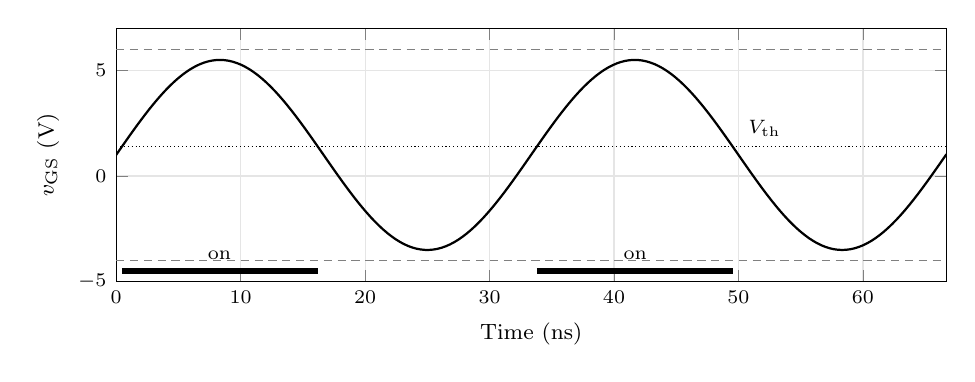
\begin{tikzpicture}
					\begin{axis}[
							width=\linewidth, height=4.8cm,
							xmin=0, xmax=66.7, ymin=-5, ymax=7,
							xlabel={Time (ns)}, ylabel={$v_\mathrm{GS}$ (V)},
							grid=major, grid style={gray!20},
							tick label style={font=\scriptsize}, label style={font=\footnotesize},
						]
						\addplot[black, thick, domain=0:66.7, samples=200] {1.0+4.5*sin(deg(2*pi*0.03*x))};
						\addplot[black, densely dotted, domain=0:66.7, samples=2] {1.4};
						\addplot[gray, densely dashed, domain=0:66.7, samples=2] {6};
						\addplot[gray, densely dashed, domain=0:66.7, samples=2] {-4};
						\draw[line width=2pt] (axis cs:0.47,-4.5) -- (axis cs:16.19,-4.5);
						\draw[line width=2pt] (axis cs:33.8,-4.5) -- (axis cs:49.53,-4.5);
						\node[font=\scriptsize, anchor=south] at (axis cs:8.3,-4.4) {on};
						\node[font=\scriptsize, anchor=south] at (axis cs:41.7,-4.4) {on};
						\node[font=\scriptsize, anchor=south west] at (axis cs:50,1.4) {$V_\mathrm{th}$};
					\end{axis}
				\end{tikzpicture}
				\caption{$v_\mathrm{GS}=1\,\mathrm{V}+4.5\,\mathrm{V}\sin\omega t$ at 30\,MHz: on for $v_\mathrm{GS}>V_\mathrm{th}=1.4$\,V, $D=0.47$; dashed: gate limits of EPC2045}
			\end{figure}
		\end{column}
		\begin{column}{0.47\textwidth}
			\footnotesize
			An inductor resonates with $C_\mathrm{iss}$: the gate energy oscillates instead of being dissipated, only $R_\mathrm{G}$ causes loss. For the same peak-to-peak voltage $V$:
			\begin{equation*}
				\frac{P_\mathrm{res}}{P_\mathrm{hard}}=\frac{\tfrac12\left(\omega C\tfrac{V}{2}\right)^2R_\mathrm{G}}{CV^2f}=\frac{\pi^2}{2}\,f\,R_\mathrm{G}\,C
			\end{equation*}
			30\,MHz, $C=Q_\mathrm{G}/V=1.4$\,nF, $R_\mathrm{G}=0.5\,\Omega$: 0.11\,W instead of 1.05\,W.
			\begin{itemize}
				\item Limits: the duty cycle is set by the DC bias of the sinusoid, and the sinusoidal edges are slow.
				\item Suited to ZVS stages (class E, $\Phi_2$), where slow gate edges cost little. Self-oscillating versions take the drive from the power stage.
			\end{itemize}
		\end{column}
	\end{columns}
	\blfootnote{Sources: Zhang and Liu, 2017, Ch.\ 2; Andersen et al., IEEE APEC 2011, pp.\ 885--891.}
\end{frame}

%%%%%%%%%%%%%%%%%%%%%%%%%%%%%%%%%%%%%%%%%%%%%%%%%%%%%%%%%%%%%
%% Integrated power stages %%
%%%%%%%%%%%%%%%%%%%%%%%%%%%%%%%%%%%%%%%%%%%%%%%%%%%%%%%%%%%%%
\begin{frame}
	\frametitle{Integrated power stages}
	\begin{table}
		\centering
		\footnotesize
		\begin{tabular}{|l|l|l|>{\raggedright\arraybackslash}p{6.4cm}|}
			\hline
			\textbf{Example} & \textbf{Integration} & \textbf{Rating}       & \textbf{Inside}                                                         \\
			\hline
			TI LMG5200       & co-packaged          & 80\,V, 10\,A          & driver and GaN half-bridge, 6\,mm $\times$ 8\,mm                        \\
			EPC2152          & monolithic           & 80\,V, 12.5\,A        & level shift, bootstrap, drivers and half-bridge, 3.9\,mm $\times$ 2.6\,mm \\
			TI LMG3410R070   & co-packaged          & 600\,V, 70\,m$\Omega$ & driver, slew rate 25--100\,V/ns, over-current response below 100\,ns    \\
			\hline
		\end{tabular}
		\caption{GaN power stages with integrated driver (manufacturer data)}
	\end{table}
	\begin{columns}[T]
		\begin{column}{0.48\textwidth}
			\small
			\textbf{Benefits}
			\begin{itemize}
				\item Gate loop and common-source inductance inside the package
				\item Matched delays, protection, less layout risk
			\end{itemize}
		\end{column}
		\begin{column}{0.49\textwidth}
			\small
			\textbf{Limits}
			\begin{itemize}
				\item Drive strength, dead time and gate voltage partly fixed by the manufacturer
				\item Driver loss heats the transistor package
				\item Fewer ratings to choose from
			\end{itemize}
		\end{column}
	\end{columns}
	\blfootnote{Sources: TI LMG5200 datasheet and LMG3410R070 product page; EPC2152 product announcement; Lidow et al., 2019, Sec.\ 3.9 and 3.11.2.}
\end{frame}

%%%%%%%%%%%%%%%%%%%%%%%%%%%%%%%%%%%%%%%%%%%%%%%%%%%%%%%%%%%%%
%% Checklist %%
%%%%%%%%%%%%%%%%%%%%%%%%%%%%%%%%%%%%%%%%%%%%%%%%%%%%%%%%%%%%%
\begin{frame}
	\frametitle{Driver checklist}
	\begin{table}
		\centering
		\footnotesize
		\begin{tabular}{|>{\raggedright\arraybackslash}p{3.6cm}|>{\raggedright\arraybackslash}p{9.6cm}|}
			\hline
			\textbf{Item}                     & \textbf{Check at MHz switching frequency}                                                                \\
			\hline
			Drive voltage and UVLO            & fits the device; UVLO above the gate voltage needed for full enhancement                                 \\
			Output stage                      & split outputs; $R_\mathrm{G,on}$ from damping and $\mathrm{d}v/\mathrm{d}t$, small $R_\mathrm{G,off}$     \\
			Delay and matching                & delay small against the period; matching of a few ns enters the dead time                               \\
			Minimum pulse width               & shorter than the shortest on-time                                                                       \\
			CMTI                              & minimum CMTI above the peak $\mathrm{d}v/\mathrm{d}t$ of the switch node                                  \\
			Floating supply                   & bootstrap: recharge time and over-charge; isolated supply: coupling capacitance                         \\
			Protection                        & over-current (desaturation or current sense), over-temperature                                           \\
			Package and layout                & low-inductance package, driver next to the transistor, supply capacitor at the pins, Kelvin source      \\
			Driver dissipation                & most of $Q_\mathrm{G}V_\mathrm{dr}f_\mathrm{sw}$ per switch, plus bias and level-shifter losses           \\
			\hline
		\end{tabular}
		\caption{Use this list for the gate-drive part of your design package (D3)}
	\end{table}
\end{frame}

%%%%%%%%%%%%%%%%%%%%%%%%%%%%%%%%%%%%%%%%%%%%%%%%%%%%%%%%%%%%%
%% Key messages %%
%%%%%%%%%%%%%%%%%%%%%%%%%%%%%%%%%%%%%%%%%%%%%%%%%%%%%%%%%%%%%
\begin{frame}
	\frametitle{Key messages}
	\begin{enumerate}
		\item An e-mode GaN gate has about 1\,V of margin. Damp the gate loop, $R_\mathrm{G}\geq2\sqrt{L_\mathrm{G}/C_\mathrm{iss}}$; a fast gate without overshoot needs a small $L_\mathrm{G}$.
		\item Turn on with a controlled $R_\mathrm{G,on}$, turn off with a small $R_\mathrm{G,off}$.
		\item Common-source inductance acts like a large extra gate resistance and steps the gate of the off-state switch: Kelvin source.
		\item Keep the off-state switch off: Miller ratio below 1, low-impedance off path, damping. Use a negative off-voltage only if the dead-time loss allows it.
		\item Bootstrap: size $C_\mathrm{boot}$ for $Q_\mathrm{tot}$, check the recharge time at maximum duty cycle and the over-charge in the dead time.
		\item At 10\,MHz delays, matching, minimum pulse width and CMTI decide; above 10\,MHz the gate power does too: resonant or integrated drive.
	\end{enumerate}
\end{frame}

%%%%%%%%%%%%%%%%%%%%%%%%%%%%%%%%%%%%%%%%%%%%%%%%%%%%%%%%%%%%%
%% Exit ticket %%
%%%%%%%%%%%%%%%%%%%%%%%%%%%%%%%%%%%%%%%%%%%%%%%%%%%%%%%%%%%%%
% Two pages: questions (page 1) and answers (page 2).
\begin{frame}<handout:1-2>
	\frametitle{Exit questions}
	\begin{varblock}[\textwidth]{Three questions, one minute each}
		\begin{enumerate}
			\item A gate loop has $L_\mathrm{G}=2$\,nH and $C_\mathrm{iss}=1$\,nF. Which total gate resistance avoids overshoot?
			\item Why does a negative off-state gate voltage increase the dead-time loss of a GaN half-bridge?
			\item A 13.56\,MHz converter uses a GaN transistor with $Q_\mathrm{G}=3$\,nC at 5\,V. Which gate-drive power does a conventional driver need?
		\end{enumerate}
	\end{varblock}
	\onslide<2-|handout:2>{
		\begin{enumerate}
			\item $R_\mathrm{G}\geq2\sqrt{2\,\mathrm{nH}/1\,\mathrm{nF}}=2.8\,\Omega$.
			\item The channel conducts in reverse when $v_\mathrm{GD}$ exceeds $V_\mathrm{th}$. $V_\mathrm{SD}$ therefore rises by $|v_\mathrm{GS,off}|$, and with it the loss $2V_\mathrm{SD}It_\mathrm{d}f_\mathrm{sw}$.
			\item $Q_\mathrm{G}V_\mathrm{dr}f_\mathrm{sw}=3\,\mathrm{nC}\cdot5\,\mathrm{V}\cdot13.56\,\mathrm{MHz}=0.2$\,W per switch.
		\end{enumerate}
	}
\end{frame}

%%%%%%%%%%%%%%%%%%%%%%%%%%%%%%%%%%%%%%%%%%%%%%%%%%%%%%%%%%%%%
%% Design project kick-off %%
%%%%%%%%%%%%%%%%%%%%%%%%%%%%%%%%%%%%%%%%%%%%%%%%%%%%%%%%%%%%%
\subsection{Design project}

\begin{frame}
	\frametitle{Project kick-off}
	\begin{columns}[T]
		\begin{column}{0.5\textwidth}
			\small
			\textbf{From today}
			\begin{itemize}
				\item Form teams of two and name two preferred briefs (B1--B6, see L1). Each team then receives its own parameter variant.
				\item Both team members must be able to defend the whole design in the oral exam.
			\end{itemize}
			\textbf{M0 on 11.11.} (voluntary, at most two pages, written feedback within a week)
			\begin{itemize}
				\item Specification sheet: ratings, operating range, efficiency target
				\item Topology justification: why this circuit at this frequency
				\item First-order loss budget
			\end{itemize}
		\end{column}
		\begin{column}{0.47\textwidth}
			\small
			\textbf{A first loss budget} (L1--L4)
			\begin{table}
				\centering
				\footnotesize
				\begin{tabular}{|l|l|}
					\hline
					conduction & $I_\mathrm{rms}^2R_\mathrm{DS(on)}$, hot and dynamic \\
					switching  & overlap and $Q_\mathrm{oss}V$, or ZVS check          \\
					dead time  & $2V_\mathrm{SD}It_\mathrm{d}f_\mathrm{sw}$            \\
					gate drive & $Q_\mathrm{G}V_\mathrm{dr}f_\mathrm{sw}$ per switch   \\
					magnetics  & estimate now, design in M1                            \\
					\hline
				\end{tabular}
			\end{table}
			Write each term as a formula with numbers, then the sum. The largest term shows where the design effort goes.
		\end{column}
	\end{columns}
\end{frame}

%%%%%%%%%%%%%%%%%%%%%%%%%%%%%%%%%%%%%%%%%%%%%%%%%%%%%%%%%%%%%
%% Gate drive in the briefs %%
%%%%%%%%%%%%%%%%%%%%%%%%%%%%%%%%%%%%%%%%%%%%%%%%%%%%%%%%%%%%%
\begin{frame}
	\frametitle{Gate drive in the briefs}
	\begin{table}
		\centering
		\footnotesize
		\begin{tabular}{|l|>{\raggedright\arraybackslash}p{3.2cm}|>{\raggedright\arraybackslash}p{9.4cm}|}
			\hline
			   & \textbf{Brief}           & \textbf{Gate-drive question}                                                                                        \\
			\hline
			B1 & ZVS GaN buck, 1--3\,MHz  & bootstrap recharge at the highest frequency; dead time over the load range, as $2Q_\mathrm{oss}/I$ varies            \\
			B2 & LLC DCX, 1\,MHz          & primary drive and timing of the synchronous rectifiers on the secondary side                                        \\
			B3 & DAB, 0.5--1\,MHz         & eight switches, floating supplies on both sides, signals across the isolation barrier (CMTI), phase-shift resolution \\
			B4 & 6.78\,MHz class E        & ground-referenced switch without bootstrap; gate power and driver dissipation (class D: high-side supply)           \\
			B5 & 13.56\,MHz VHF           & period 73.75\,ns; gate power is a large part of 5--10\,W, resonant drive is an option                                 \\
			B6 & hybrid SC, 48\,V         & switches at several floating potentials: cascaded bootstrap or isolated supplies                                    \\
			\hline
		\end{tabular}
		\caption{Every design package contains a gate-drive design with timing budget (D3, reviewed at M2)}
	\end{table}
\end{frame}

%%%%%%%%%%%%%%%%%%%%%%%%%%%%%%%%%%%%%%%%%%%%%%%%%%%%%%%%%%%%%
%% References %%
%%%%%%%%%%%%%%%%%%%%%%%%%%%%%%%%%%%%%%%%%%%%%%%%%%%%%%%%%%%%%
\begin{frame}
	\frametitle{References}
	\scriptsize
	\begin{itemize}
		\item A. Lidow, M. de Rooij, J. Strydom, D. Reusch, J. Glaser, \textit{GaN Transistors for Efficient Power Conversion}, 3rd ed., Wiley, 2019, Ch.\ 2 and 3.
		\item Z. Zhang, Y.-F. Liu, \textit{High Frequency MOSFET Gate Drivers: Technologies and Applications}, IET, 2017.
		\item F. Wang, Z. Zhang, E.\,A. Jones, \textit{Characterization of Wide Bandgap Power Semiconductor Devices}, IET, 2018, Ch.\ 5 and 7.
		\item D. Reusch, M. de Rooij, ``Evaluation of gate drive overvoltage management methods for enhancement mode gallium nitride transistors,'' IEEE APEC 2017, pp.\ 2459--2466.
		\item T.\,M. Andersen, S.\,K. Christensen, A. Knott, M. Andersen, ``A VHF class E DC--DC converter with self-oscillating gate driver,'' IEEE APEC 2011, pp.\ 885--891.
		\item D.\,J. Perreault, \textit{6.622 Power Electronics}, Lecture 38: Gate drive, level shift, layout, MIT OpenCourseWare, Spring 2023.
		\item JEDEC JEP184, \textit{Guideline for Evaluating Bias Temperature Instability of Silicon Carbide Metal-Oxide-Semiconductor Devices for Power Electronic Conversion}, 2021.
		\item N. Mehta, ``Design considerations for LMG1205 advanced GaN FET driver during high-frequency operation,'' TI application report SNVA723A, 2018.
		\item Datasheets: EPC2045, EPC2152, LMG1205, LMG1210, LMG5200, LMG3410R070, ADuM4120, C2M0280120D, C3M0065090D.
	\end{itemize}
\end{frame}
